\head{Февраль}{Листок 5. Теория множеств. Уровень 1.}

\begin{thm}
Докажите, что для любых множеств $A$, $B$ и $C$ справедливы соотношения:
\par
а)~$(A \cap B) \cup C = (A \cup C) \cap (B \cup C)$;
б)~$(A \cap B) \backslash C = (A \backslash C) \cap (B \backslash C)$
\end{thm}

\begin{thm}
При каких условиях множества $A$ и $B$ справедливы следующие соотношения:
\par
а)~$A \backslash B = A$; \hfill
б)~$A \backslash B = B$; \hfill
в)~$A \cup B = A$; \hfill
г)~$A \cap B = A$; 
\par
д)~$A \backslash B = B \backslash A$; \hfill
е)~$A \cup B = A \cap B$; \hfill
ж)~$A \cup B = A \backslash B$; \hfill
з)~$A \cap B = A \backslash B$~?
\end{thm}



{\setlength{\intextsep}{2pt}
\begin{figure}[h]
\begin{minipage}{0.8\linewidth}\setlength{\parindent}{1.5em}
\begin{thm}
Известно, что $A = B \cup C$. Верно ли тогда, что $A \backslash B = C$?
\end{thm}

\begin{thm}
Известно, что $A \backslash B = C$. Верно ли тогда, что $A = B \cup C$?
\end{thm}

\begin{thm}
Известно, что $A \subset B \cup C$, $B \subset A \cup C$, $C \subset A \cup B$. Следует ли отсюда, что $A = B = C$?
\end{thm}
    \begin{thm}
    Даны четыре множества $A$, $B$, $C$ и $D$, изображённые на рисунке справа. При помощи операций $\cap$, $\cup$, $\backslash$ и $\Delta$ выразите закрашенное множество $M$ через $A$, $B$, $C$ и $D$.\footnotemark
    \end{thm}
\end{minipage}
\hfill
\begin{minipage}{0.17\linewidth}
    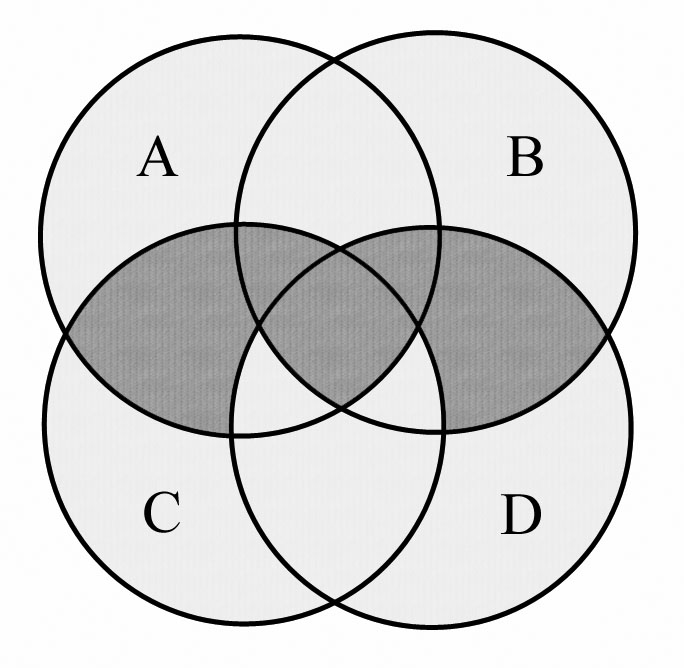
\includegraphics[width=0.9\columnwidth]{img/euler3.png}
\end{minipage}
\end{figure}}\footnotetext{Лёня утверждает, что $M$ можно выразить, использовав лишь 6 операций! За сколько операций это сделаете Вы?}

\section{Метод ''кругов Эйлера''}

\begin{thm}
Из 42 хемулей 17 собирают пуговицы, а 29 очень любят сладкое. При этом 13 хемулей не
интересуются ни сластями, ни пуговицами. Сколько сладкоежек собирают пуговицы?
\end{thm}

\begin{thm}
Три лентяя красили пол в комнате площадью $12м^2$. Сначала один покрасил $5м^2$ синей краской, затем второй – $4м^2$ красной краской и, наконец, третий – $3м^2$ желтой. В результате оказалось, что любыми двумя цветами покрашена площадь в $1,5м^2$, а $0,5м^2$ покрашена всеми тремя цветами. 
\par
Какая площадь пола покрашена в синий цвет? Какова площадь неокрашенного пола?
\end{thm}

\begin{thm}
В классе послушных девочек столько же, сколько непослушных мальчиков. Кого в классе
больше: послушных детей или мальчиков?
\end{thm}

{\setlength{\intextsep}{2pt}
\begin{figure}[h]
\begin{minipage}{0.85\linewidth}\setlength{\parindent}{1.5em}
    \begin{thm}
    В Швейцарии 95\% населения знают немецкий язык, 80\% – французский, а 75\% – английский или итальянский. Сколько процентов населения заведомо владеет тремя языками?
    \end{thm}

    \begin{thm}
    В семье крестьянина семеро детей любят капусту, шестеро – морковь, пятеро – горох, четверо – капусту и морковь, трое – капусту и горох, двое – морковь и горох, а один любит всё. Сколько всего детей в семье крестьянина (если нет таких, кто не любит ни капусту, ни морковь, ни горох)?
    \end{thm}
\end{minipage}
\hfill
\begin{minipage}{0.14\linewidth}
    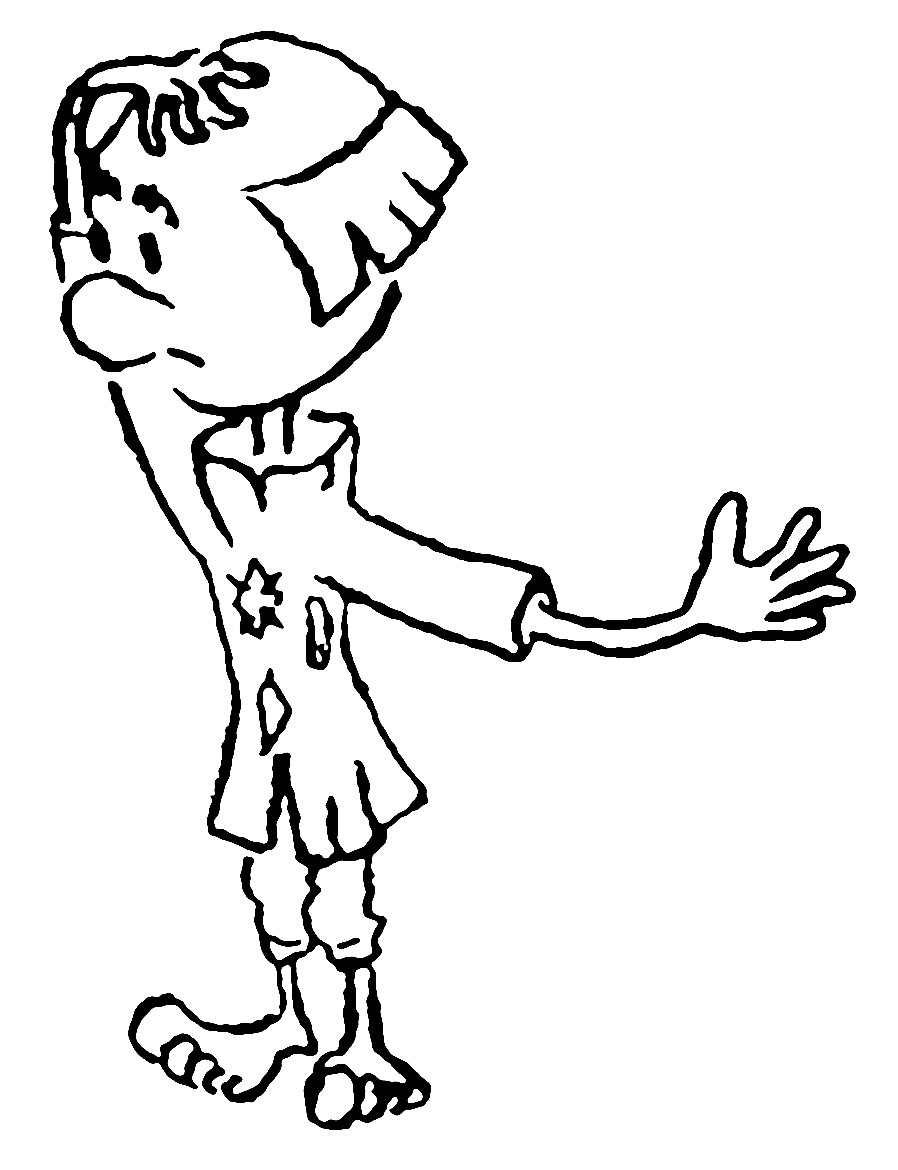
\includegraphics[width=0.95\columnwidth]{img/krestyanin.png}
\end{minipage}
\end{figure}}

\begin{thm}
На пиратском корабле трудятся 67 морских разбойников. У 47 из них есть ухо, у 35 – глаз, а у 23 счастливчиков есть и то, и другое. Новая инструкция Профсоюза Работников Абордажного Крюка предписывает корабельному врачу учитывать также наличие носа. Оказалось, что 20 пиратов имеют нос, 12 – и нос, и ухо, 11 – и нос, и глаз, а 5 – все три органа. Сколько пиратов не имеют ничего?
\end{thm}

\begin{thm}
Все животные старухи Шапокляк, кроме двух, – кошки; все, кроме двух – собаки; и все, кроме
двух – попугаи, а остальные – тараканы. Сколько всего животных у старухи Шапокляк? Какие именно это животные?
\end{thm}